\section{Complete Simulation Results}
\label{appendix:simulation}

\begin{table}
\renewcommand{\arraystretch}{1.2}
  \centering
  \begin{tabular}{ | c | c | c | c | c | }
    \hline
    Scenario        & Time? &  \paramtt{} (s)   & \paramteff{} (s)   & \paramtprl{} (s)  \\
    \hline
    \hline
    A1              & no                  & 30                & 60                 & 30                \\
    \hline
    A2              & no                  & 150               & 300                & 150               \\
    \hline
    B1              & yes                 & 30                & 60                 & 30                \\
    \hline
    B2              & yes                 & 150               & 300                & 150               \\
    \hline
  \end{tabular}
  \vspace{0.2cm}
  \caption{ Scenarios evaluated in our simulation. Parameters are chosen
  according to the desired \paramteff{}. The column named \emph{Time?} indicates
  whether a local trusted time source is used in \acp{TC} or not.}
  \label{tbl:eval-scenarios}
  %\vspace{-5mm}
\end{table}
%




\begin{figure}[t]
    %\centering
    \hspace*{-0.3cm}
    \resizebox{1.05\linewidth}{!} {
      % This file was created with tikzplotlib v0.10.1.
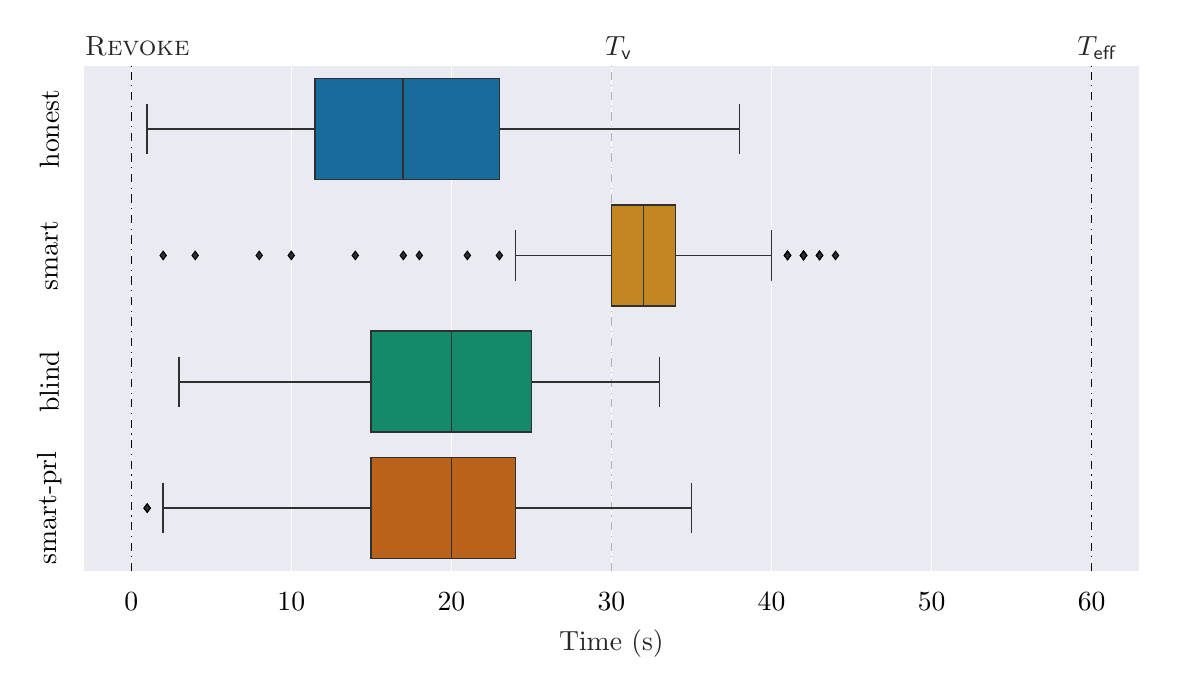
\begin{tikzpicture}

\definecolor{chocolate1869726}{RGB}{186,97,26}
\definecolor{darkgoldenrod19413532}{RGB}{194,135,32}
\definecolor{darkslategray38}{RGB}{38,38,38}
\definecolor{darkslategray48}{RGB}{48,48,48}
\definecolor{lavender234234242}{RGB}{234,234,242}
\definecolor{seagreen21138106}{RGB}{21,138,106}
\definecolor{teal23108155}{RGB}{23,108,155}

\begin{axis}[
clip=false,
axis background/.style={fill=lavender234234242},
axis line style={white},
height=8cm,
minor xtick={},
minor ytick={},
tick align=outside,
width=15cm,
x grid style={white},
xlabel=\textcolor{darkslategray38}{Time (s)},
xmajorgrids,
xmajorticks=true,
xmin=-3, xmax=63,
xtick style={color=darkslategray38,draw=none},
xtick={-10,0,10,20,30,40,50,60,70},
y dir=reverse,
y grid style={white},
ymajorticks=true,
ymin=-0.5, ymax=3.5,
ytick style={color=darkslategray38,draw=none},
ytick={0,1,2,3},
yticklabel style={rotate=90.0,anchor=center,yshift=8pt},
yticklabels={honest,smart,blind,smart-prl}
]
% START VERTICAL LINES %
\addplot [dashdotted, black]
table {%
0 3.5
0 -0.5
};
\addplot [dashdotted, gray!60]
table {%
30 3.5
30 -0.5
};
\addplot [dashdotted, black]
table {%
60 3.5
60 -0.5
};
% END VERTICAL LINES %
\path [draw=darkslategray48, fill=teal23108155, semithick]
(axis cs:11.5,-0.4)
--(axis cs:11.5,0.4)
--(axis cs:23,0.4)
--(axis cs:23,-0.4)
--(axis cs:11.5,-0.4)
--cycle;
\path [draw=darkslategray48, fill=darkgoldenrod19413532, semithick]
(axis cs:30,0.6)
--(axis cs:30,1.4)
--(axis cs:34,1.4)
--(axis cs:34,0.6)
--(axis cs:30,0.6)
--cycle;
\path [draw=darkslategray48, fill=seagreen21138106, semithick]
(axis cs:15,1.6)
--(axis cs:15,2.4)
--(axis cs:25,2.4)
--(axis cs:25,1.6)
--(axis cs:15,1.6)
--cycle;
\path [draw=darkslategray48, fill=chocolate1869726, semithick]
(axis cs:15,2.6)
--(axis cs:15,3.4)
--(axis cs:24,3.4)
--(axis cs:24,2.6)
--(axis cs:15,2.6)
--cycle;
\addplot [semithick, darkslategray48]
table {%
11.5 0
1 0
};
\addplot [semithick, darkslategray48]
table {%
23 0
38 0
};
\addplot [semithick, darkslategray48]
table {%
1 -0.2
1 0.2
};
\addplot [semithick, darkslategray48]
table {%
38 -0.2
38 0.2
};
\addplot [semithick, darkslategray48]
table {%
30 1
24 1
};
\addplot [semithick, darkslategray48]
table {%
34 1
40 1
};
\addplot [semithick, darkslategray48]
table {%
24 0.8
24 1.2
};
\addplot [semithick, darkslategray48]
table {%
40 0.8
40 1.2
};
\addplot [black, mark=diamond*, mark size=1.5, mark options={solid,fill=darkslategray48}, only marks]
table {%
2 1
23 1
10 1
18 1
14 1
4 1
8 1
17 1
21 1
44 1
43 1
41 1
42 1
41 1
42 1
43 1
41 1
43 1
42 1
42 1
};
\addplot [semithick, darkslategray48]
table {%
15 2
3 2
};
\addplot [semithick, darkslategray48]
table {%
25 2
33 2
};
\addplot [semithick, darkslategray48]
table {%
3 1.8
3 2.2
};
\addplot [semithick, darkslategray48]
table {%
33 1.8
33 2.2
};
\addplot [semithick, darkslategray48]
table {%
15 3
2 3
};
\addplot [semithick, darkslategray48]
table {%
24 3
35 3
};
\addplot [semithick, darkslategray48]
table {%
2 2.8
2 3.2
};
\addplot [semithick, darkslategray48]
table {%
35 2.8
35 3.2
};
\addplot [black, mark=diamond*, mark size=1.5, mark options={solid,fill=darkslategray48}, only marks]
table {%
1 3
1 3
};
\addplot [semithick, darkslategray48]
table {%
17 -0.4
17 0.4
};
\addplot [semithick, darkslategray48]
table {%
32 0.6
32 1.4
};
\addplot [semithick, darkslategray48]
table {%
20 1.6
20 2.4
};
\addplot [semithick, darkslategray48]
table {%
20 2.6
20 3.4
};
\draw (axis cs:-3.5,-0.58) node[
  scale=1,
  anchor=base west,
  text=darkslategray38,
  rotate=0.0
]{\textsc{Revoke}};
\draw[dashed] (axis cs:29,-0.58) node[
  scale=1,
  anchor=base west,
  text=darkslategray38,
  rotate=0.0
]{$T_{\mathsf{v}}$};
\draw (axis cs:58.5,-0.58) node[
  scale=1,
  anchor=base west,
  text=darkslategray38,
  rotate=0.0
]{$T_{\mathsf{eff}}$};
\end{axis}

\end{tikzpicture}

    } \caption{Simulation results for scenario A1.}
    \label{fig:eval-sim-a1}
\end{figure}

\begin{figure}[t]
    %\centering
    \hspace*{-0.3cm}
    \resizebox{1.05\linewidth}{!} {
      % This file was created with tikzplotlib v0.10.1.
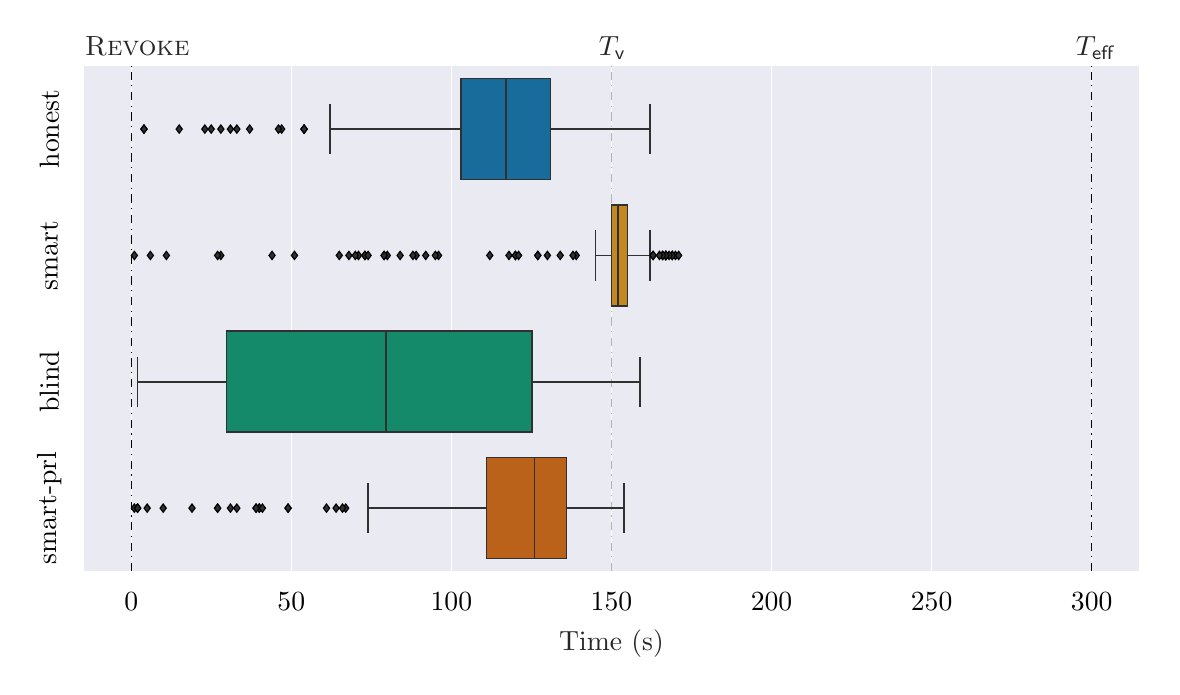
\begin{tikzpicture}

\definecolor{chocolate1869726}{RGB}{186,97,26}
\definecolor{darkgoldenrod19413532}{RGB}{194,135,32}
\definecolor{darkslategray38}{RGB}{38,38,38}
\definecolor{darkslategray48}{RGB}{48,48,48}
\definecolor{lavender234234242}{RGB}{234,234,242}
\definecolor{seagreen21138106}{RGB}{21,138,106}
\definecolor{teal23108155}{RGB}{23,108,155}

\begin{axis}[
clip=false,
axis background/.style={fill=lavender234234242},
axis line style={white},
height=8cm,
minor xtick={},
minor ytick={},
tick align=outside,
width=15cm,
x grid style={white},
xlabel=\textcolor{darkslategray38}{Time (s)},
xmajorgrids,
xmajorticks=true,
xmin=-15, xmax=315,
xtick style={color=darkslategray38,draw=none},
xtick={-50,0,50,100,150,200,250,300,350},
y dir=reverse,
y grid style={white},
ymajorticks=true,
ymin=-0.5, ymax=3.5,
ytick style={color=darkslategray38,draw=none},
ytick={0,1,2,3},
yticklabel style={rotate=90.0,anchor=center,yshift=8pt},
yticklabels={honest,smart,blind,smart-prl}
]
% START VERTICAL LINES %
\addplot [dashdotted, black]
table {%
0 3.5
0 -0.5
};
\addplot [dashdotted, gray!60]
table {%
150 3.5
150 -0.5
};
\addplot [dashdotted, black]
table {%
300 3.5
300 -0.5
};
% END VERTICAL LINES %
\path [draw=darkslategray48, fill=teal23108155, semithick]
(axis cs:103,-0.4)
--(axis cs:103,0.4)
--(axis cs:131,0.4)
--(axis cs:131,-0.4)
--(axis cs:103,-0.4)
--cycle;
\path [draw=darkslategray48, fill=darkgoldenrod19413532, semithick]
(axis cs:150,0.6)
--(axis cs:150,1.4)
--(axis cs:155,1.4)
--(axis cs:155,0.6)
--(axis cs:150,0.6)
--cycle;
\path [draw=darkslategray48, fill=seagreen21138106, semithick]
(axis cs:29.75,1.6)
--(axis cs:29.75,2.4)
--(axis cs:125.25,2.4)
--(axis cs:125.25,1.6)
--(axis cs:29.75,1.6)
--cycle;
\path [draw=darkslategray48, fill=chocolate1869726, semithick]
(axis cs:111,2.6)
--(axis cs:111,3.4)
--(axis cs:136,3.4)
--(axis cs:136,2.6)
--(axis cs:111,2.6)
--cycle;
\addplot [semithick, darkslategray48]
table {%
103 0
62 0
};
\addplot [semithick, darkslategray48]
table {%
131 0
162 0
};
\addplot [semithick, darkslategray48]
table {%
62 -0.2
62 0.2
};
\addplot [semithick, darkslategray48]
table {%
162 -0.2
162 0.2
};
\addplot [black, mark=diamond*, mark size=1.5, mark options={solid,fill=darkslategray48}, only marks]
table {%
4 0
15 0
31 0
33 0
4 0
37 0
25 0
47 0
28 0
54 0
23 0
54 0
46 0
54 0
};
\addplot [semithick, darkslategray48]
table {%
150 1
145 1
};
\addplot [semithick, darkslategray48]
table {%
155 1
162 1
};
\addplot [semithick, darkslategray48]
table {%
145 0.8
145 1.2
};
\addplot [semithick, darkslategray48]
table {%
162 0.8
162 1.2
};
\addplot [black, mark=diamond*, mark size=1.5, mark options={solid,fill=darkslategray48}, only marks]
table {%
127 1
73 1
89 1
96 1
84 1
118 1
80 1
134 1
28 1
79 1
120 1
127 1
120 1
51 1
130 1
65 1
88 1
71 1
112 1
68 1
27 1
73 1
79 1
44 1
74 1
1 1
121 1
6 1
95 1
92 1
139 1
70 1
138 1
11 1
167 1
166 1
169 1
163 1
170 1
167 1
167 1
169 1
168 1
167 1
167 1
166 1
163 1
171 1
165 1
};
\addplot [semithick, darkslategray48]
table {%
29.75 2
2 2
};
\addplot [semithick, darkslategray48]
table {%
125.25 2
159 2
};
\addplot [semithick, darkslategray48]
table {%
2 1.8
2 2.2
};
\addplot [semithick, darkslategray48]
table {%
159 1.8
159 2.2
};
\addplot [semithick, darkslategray48]
table {%
111 3
74 3
};
\addplot [semithick, darkslategray48]
table {%
136 3
154 3
};
\addplot [semithick, darkslategray48]
table {%
74 2.8
74 3.2
};
\addplot [semithick, darkslategray48]
table {%
154 2.8
154 3.2
};
\addplot [black, mark=diamond*, mark size=1.5, mark options={solid,fill=darkslategray48}, only marks]
table {%
1 3
61 3
27 3
40 3
27 3
2 3
64 3
49 3
67 3
19 3
2 3
2 3
10 3
31 3
39 3
66 3
33 3
40 3
41 3
39 3
49 3
5 3
};
\addplot [semithick, darkslategray48]
table {%
117 -0.4
117 0.4
};
\addplot [semithick, darkslategray48]
table {%
152 0.6
152 1.4
};
\addplot [semithick, darkslategray48]
table {%
79.5 1.6
79.5 2.4
};
\addplot [semithick, darkslategray48]
table {%
126 2.6
126 3.4
};
\draw (axis cs:-17.5,-0.58) node[
  scale=1,
  anchor=base west,
  text=darkslategray38,
  rotate=0.0
]{\textsc{Revoke}};
\draw[dashed] (axis cs:143,-0.58) node[
  scale=1,
  anchor=base west,
  text=darkslategray38,
  rotate=0.0
]{$T_{\mathsf{v}}$};
\draw (axis cs:292,-0.58) node[
  scale=1,
  anchor=base west,
  text=darkslategray38,
  rotate=0.0
]{$T_{\mathsf{eff}}$};
\end{axis}

\end{tikzpicture}

    } \caption{Simulation results for scenario A2.}
    \label{fig:eval-sim-a2}
\end{figure}

\begin{figure}[t]
    %\centering
    \hspace*{-0.3cm}
    \resizebox{1.05\linewidth}{!} {
      % This file was created with tikzplotlib v0.10.1.
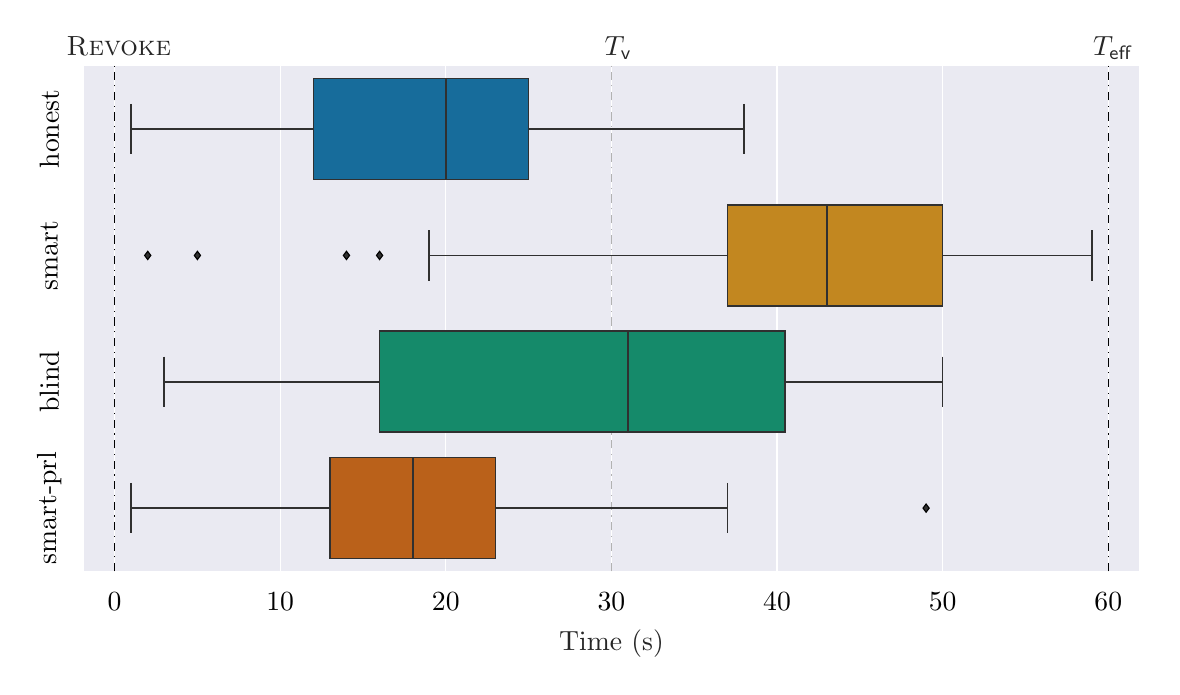
\begin{tikzpicture}

\definecolor{chocolate1869726}{RGB}{186,97,26}
\definecolor{darkgoldenrod19413532}{RGB}{194,135,32}
\definecolor{darkslategray38}{RGB}{38,38,38}
\definecolor{darkslategray48}{RGB}{48,48,48}
\definecolor{lavender234234242}{RGB}{234,234,242}
\definecolor{seagreen21138106}{RGB}{21,138,106}
\definecolor{teal23108155}{RGB}{23,108,155}

\begin{axis}[
clip=false,
axis background/.style={fill=lavender234234242},
axis line style={white},
height=8cm,
minor xtick={},
minor ytick={},
tick align=outside,
width=15cm,
x grid style={white},
xlabel=\textcolor{darkslategray38}{Time (s)},
xmajorgrids,
xmajorticks=true,
xmin=-1.9, xmax=61.9,
xtick style={color=darkslategray38,draw=none},
xtick={-10,0,10,20,30,40,50,60,70},
y dir=reverse,
y grid style={white},
ymajorticks=true,
ymin=-0.5, ymax=3.5,
ytick style={color=darkslategray38,draw=none},
ytick={0,1,2,3},
yticklabel style={rotate=90.0,anchor=center,yshift=8pt},
yticklabels={honest,smart,blind,smart-prl}
]
% START VERTICAL LINES %
\addplot [dashdotted, black]
table {%
0 3.5
0 -0.5
};
\addplot [dashdotted, gray!60]
table {%
30 3.5
30 -0.5
};
\addplot [dashdotted, black]
table {%
60 3.5
60 -0.5
};
% END VERTICAL LINES %
\path [draw=darkslategray48, fill=teal23108155, semithick]
(axis cs:12,-0.4)
--(axis cs:12,0.4)
--(axis cs:25,0.4)
--(axis cs:25,-0.4)
--(axis cs:12,-0.4)
--cycle;
\path [draw=darkslategray48, fill=darkgoldenrod19413532, semithick]
(axis cs:37,0.6)
--(axis cs:37,1.4)
--(axis cs:50,1.4)
--(axis cs:50,0.6)
--(axis cs:37,0.6)
--cycle;
\path [draw=darkslategray48, fill=seagreen21138106, semithick]
(axis cs:16,1.6)
--(axis cs:16,2.4)
--(axis cs:40.5,2.4)
--(axis cs:40.5,1.6)
--(axis cs:16,1.6)
--cycle;
\path [draw=darkslategray48, fill=chocolate1869726, semithick]
(axis cs:13,2.6)
--(axis cs:13,3.4)
--(axis cs:23,3.4)
--(axis cs:23,2.6)
--(axis cs:13,2.6)
--cycle;
\addplot [semithick, darkslategray48]
table {%
12 0
1 0
};
\addplot [semithick, darkslategray48]
table {%
25 0
38 0
};
\addplot [semithick, darkslategray48]
table {%
1 -0.2
1 0.2
};
\addplot [semithick, darkslategray48]
table {%
38 -0.2
38 0.2
};
\addplot [semithick, darkslategray48]
table {%
37 1
19 1
};
\addplot [semithick, darkslategray48]
table {%
50 1
59 1
};
\addplot [semithick, darkslategray48]
table {%
19 0.8
19 1.2
};
\addplot [semithick, darkslategray48]
table {%
59 0.8
59 1.2
};
\addplot [black, mark=diamond*, mark size=1.5, mark options={solid,fill=darkslategray48}, only marks]
table {%
2 1
5 1
16 1
14 1
};
\addplot [semithick, darkslategray48]
table {%
16 2
3 2
};
\addplot [semithick, darkslategray48]
table {%
40.5 2
50 2
};
\addplot [semithick, darkslategray48]
table {%
3 1.8
3 2.2
};
\addplot [semithick, darkslategray48]
table {%
50 1.8
50 2.2
};
\addplot [semithick, darkslategray48]
table {%
13 3
1 3
};
\addplot [semithick, darkslategray48]
table {%
23 3
37 3
};
\addplot [semithick, darkslategray48]
table {%
1 2.8
1 3.2
};
\addplot [semithick, darkslategray48]
table {%
37 2.8
37 3.2
};
\addplot [black, mark=diamond*, mark size=1.5, mark options={solid,fill=darkslategray48}, only marks]
table {%
49 3
};
\addplot [semithick, darkslategray48]
table {%
20 -0.4
20 0.4
};
\addplot [semithick, darkslategray48]
table {%
43 0.6
43 1.4
};
\addplot [semithick, darkslategray48]
table {%
31 1.6
31 2.4
};
\addplot [semithick, darkslategray48]
table {%
18 2.6
18 3.4
};
\draw (axis cs:-3.5,-0.58) node[
  scale=1,
  anchor=base west,
  text=darkslategray38,
  rotate=0.0
]{\textsc{Revoke}};
\draw[dashed] (axis cs:29,-0.58) node[
  scale=1,
  anchor=base west,
  text=darkslategray38,
  rotate=0.0
]{$T_{\mathsf{v}}$};
\draw (axis cs:58.5,-0.58) node[
  scale=1,
  anchor=base west,
  text=darkslategray38,
  rotate=0.0
]{$T_{\mathsf{eff}}$};
\end{axis}

\end{tikzpicture}

    } \caption{Simulation results for scenario B1.}
    \label{fig:eval-sim-b1}
\end{figure}

\begin{figure}[t]
    %\centering
    \hspace*{-0.3cm}
    \resizebox{1.05\linewidth}{!} {
      % This file was created with tikzplotlib v0.10.1.
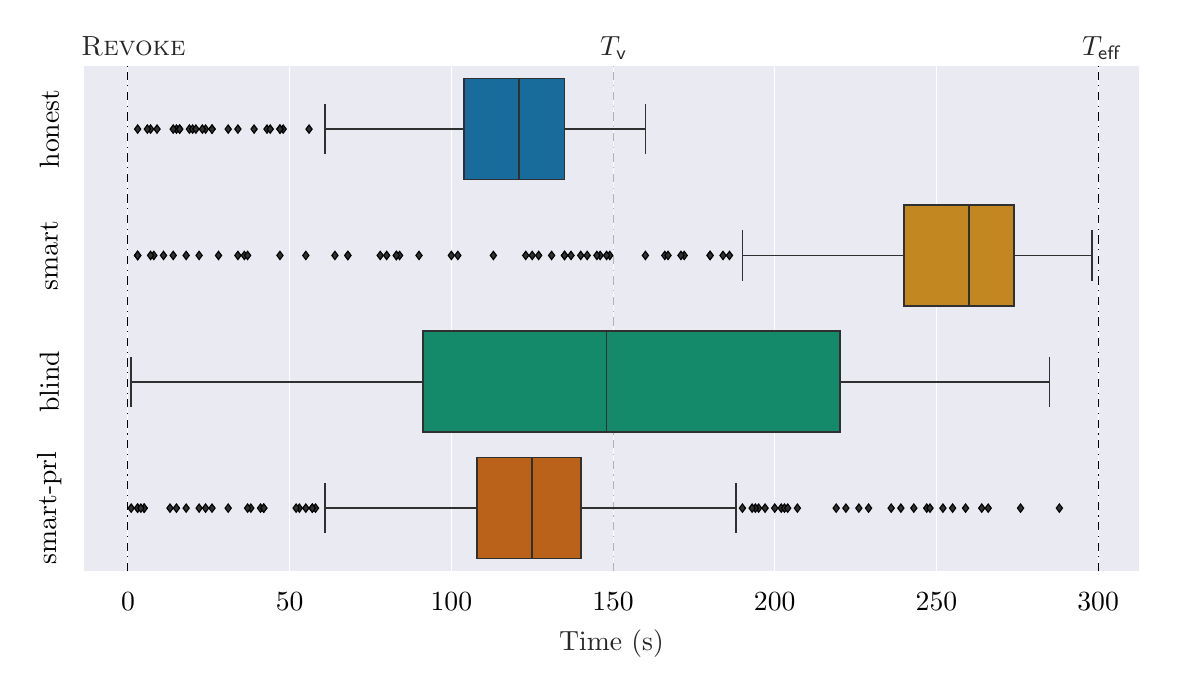
\begin{tikzpicture}

\definecolor{chocolate1869726}{RGB}{186,97,26}
\definecolor{darkgoldenrod19413532}{RGB}{194,135,32}
\definecolor{darkslategray38}{RGB}{38,38,38}
\definecolor{darkslategray48}{RGB}{48,48,48}
\definecolor{lavender234234242}{RGB}{234,234,242}
\definecolor{seagreen21138106}{RGB}{21,138,106}
\definecolor{teal23108155}{RGB}{23,108,155}

\begin{axis}[
clip=false,
axis background/.style={fill=lavender234234242},
axis line style={white},
height=8cm,
minor xtick={},
minor ytick={},
tick align=outside,
width=15cm,
x grid style={white},
xlabel=\textcolor{darkslategray38}{Time (s)},
xmajorgrids,
xmajorticks=true,
xmin=-13.85, xmax=312.85,
xtick style={color=darkslategray38,draw=none},
xtick={-50,0,50,100,150,200,250,300,350},
y dir=reverse,
y grid style={white},
ymajorticks=true,
ymin=-0.5, ymax=3.5,
ytick style={color=darkslategray38,draw=none},
ytick={0,1,2,3},
yticklabel style={rotate=90.0,anchor=center,yshift=8pt},
yticklabels={honest,smart,blind,smart-prl}
]
% START VERTICAL LINES %
\addplot [dashdotted, black]
table {%
0 3.5
0 -0.5
};
\addplot [dashdotted, gray!60]
table {%
150 3.5
150 -0.5
};
\addplot [dashdotted, black]
table {%
300 3.5
300 -0.5
};
% END VERTICAL LINES %
\path [draw=darkslategray48, fill=teal23108155, semithick]
(axis cs:104,-0.4)
--(axis cs:104,0.4)
--(axis cs:135,0.4)
--(axis cs:135,-0.4)
--(axis cs:104,-0.4)
--cycle;
\path [draw=darkslategray48, fill=darkgoldenrod19413532, semithick]
(axis cs:240,0.6)
--(axis cs:240,1.4)
--(axis cs:274,1.4)
--(axis cs:274,0.6)
--(axis cs:240,0.6)
--cycle;
\path [draw=darkslategray48, fill=seagreen21138106, semithick]
(axis cs:91.25,1.6)
--(axis cs:91.25,2.4)
--(axis cs:220.25,2.4)
--(axis cs:220.25,1.6)
--(axis cs:91.25,1.6)
--cycle;
\path [draw=darkslategray48, fill=chocolate1869726, semithick]
(axis cs:108,2.6)
--(axis cs:108,3.4)
--(axis cs:140,3.4)
--(axis cs:140,2.6)
--(axis cs:108,2.6)
--cycle;
\addplot [semithick, darkslategray48]
table {%
104 0
61 0
};
\addplot [semithick, darkslategray48]
table {%
135 0
160 0
};
\addplot [semithick, darkslategray48]
table {%
61 -0.2
61 0.2
};
\addplot [semithick, darkslategray48]
table {%
160 -0.2
160 0.2
};
\addplot [black, mark=diamond*, mark size=1.5, mark options={solid,fill=darkslategray48}, only marks]
table {%
3 0
26 0
48 0
7 0
19 0
15 0
47 0
31 0
6 0
9 0
20 0
39 0
47 0
34 0
26 0
43 0
24 0
56 0
44 0
14 0
16 0
21 0
23 0
16 0
};
\addplot [semithick, darkslategray48]
table {%
240 1
190 1
};
\addplot [semithick, darkslategray48]
table {%
274 1
298 1
};
\addplot [semithick, darkslategray48]
table {%
190 0.8
190 1.2
};
\addplot [semithick, darkslategray48]
table {%
298 0.8
298 1.2
};
\addplot [black, mark=diamond*, mark size=1.5, mark options={solid,fill=darkslategray48}, only marks]
table {%
135 1
127 1
3 1
68 1
90 1
180 1
113 1
149 1
123 1
186 1
83 1
180 1
146 1
137 1
166 1
8 1
7 1
78 1
3 1
160 1
28 1
64 1
22 1
68 1
125 1
47 1
172 1
140 1
36 1
55 1
148 1
80 1
171 1
145 1
3 1
102 1
14 1
184 1
18 1
34 1
100 1
84 1
11 1
142 1
131 1
83 1
37 1
135 1
167 1
};
\addplot [semithick, darkslategray48]
table {%
91.25 2
1 2
};
\addplot [semithick, darkslategray48]
table {%
220.25 2
285 2
};
\addplot [semithick, darkslategray48]
table {%
1 1.8
1 2.2
};
\addplot [semithick, darkslategray48]
table {%
285 1.8
285 2.2
};
\addplot [semithick, darkslategray48]
table {%
108 3
61 3
};
\addplot [semithick, darkslategray48]
table {%
140 3
188 3
};
\addplot [semithick, darkslategray48]
table {%
61 2.8
61 3.2
};
\addplot [semithick, darkslategray48]
table {%
188 2.8
188 3.2
};
\addplot [black, mark=diamond*, mark size=1.5, mark options={solid,fill=darkslategray48}, only marks]
table {%
42 3
57 3
31 3
3 3
5 3
22 3
26 3
13 3
5 3
18 3
58 3
1 3
3 3
41 3
4 3
24 3
42 3
55 3
57 3
38 3
53 3
15 3
52 3
37 3
276 3
202 3
222 3
229 3
195 3
219 3
194 3
193 3
264 3
266 3
236 3
207 3
200 3
226 3
259 3
247 3
203 3
204 3
243 3
248 3
239 3
288 3
197 3
252 3
255 3
190 3
};
\addplot [semithick, darkslategray48]
table {%
121 -0.4
121 0.4
};
\addplot [semithick, darkslategray48]
table {%
260 0.6
260 1.4
};
\addplot [semithick, darkslategray48]
table {%
148 1.6
148 2.4
};
\addplot [semithick, darkslategray48]
table {%
125 2.6
125 3.4
};
\draw (axis cs:-17.5,-0.58) node[
  scale=1,
  anchor=base west,
  text=darkslategray38,
  rotate=0.0
]{\textsc{Revoke}};
\draw[dashed] (axis cs:143,-0.58) node[
  scale=1,
  anchor=base west,
  text=darkslategray38,
  rotate=0.0
]{$T_{\mathsf{v}}$};
\draw (axis cs:292,-0.58) node[
  scale=1,
  anchor=base west,
  text=darkslategray38,
  rotate=0.0
]{$T_{\mathsf{eff}}$};
\end{axis}

\end{tikzpicture}

    } \caption{Simulation results for scenario B2.}
    \label{fig:eval-sim-b2}
\end{figure}

We ran simulations for each of the scenarios described in
\cref{tbl:eval-scenarios}. Results are depicted in
\cref{fig:eval-sim-a1,fig:eval-sim-a2,fig:eval-sim-b1,fig:eval-sim-b2}.

Recall from \cref{section:eval-sim} that each value of the boxes represents the
time between the revocation of \ps{} (\funcrevokedaa{} event) and the last
\ac{V2V} message signed with \ps{} that was verified by a non-malicious \ac{TC}
(\funcverify{} event). The latter time represents the \emph{effective revocation
time} for that particular pseudonym \ps. The box plots give the distribution of
such values, obtained aggregating more than 600 revocations, filtering out
negative values.

The figures show one significant difference between the main design (A1 and A2)
and the extension with a local trusted time source (B1 and B2): While in the
former most revocations are effective around or before \paramtt{}, in the latter
attackers are able to postpone revocation up until \paramteff{} in some cases,
i.e., it appears easier to reach the upper bound, especially for powerful
attackers such as the \attackersmart{} one. This is due to the fact that, while
in the main design revoked \acp{TC} cannot synchronize their time since
\paramtrev, with a local time source \acp{TC} can still advance their internal
time up until $\paramtrev + \paramtt$, before triggering the automatic
revocation logic. That is, in the latter case a revoked \ac{TC} is able to
generate ''more fresh'' \ac{V2V} messages, which can be processed by other
\acp{TC} later in time.

This peculiarity suggests that a local trusted time source negatively affects
the revocation time. While this may be true in the average case, it still does
not affect the worst-case effective revocation time \paramteff, as shown in the
figures.